\documentclass[a4paper, 10pt]{article}
\usepackage[utf8]{inputenc} % Change according your file encoding
\usepackage{graphicx}
\usepackage{url}

%opening
\title{Seminar Report: Groupy}
\date{\normalsize\today{}}

\begin{document}
\author{}
\maketitle

\begin{center}
  \textbf{Carles Tornel}\\
  \textbf{Jesus Alfaro}\\
  \textbf{Ricard Abril}

\end{center}
\section{Introduction}

En aquesta pràctica haurem d'implementar un servei multicast on un únic procés serà el líder del sistema i al qual els altres processos enviaran un missatge cada cop que vulguin enviar missatges multicast.
La presencia del líder fa que el sistema tingui un ordre, també serà el que tingui constància dels processos que estan actius al sistema i l'únic que fa el multicast.
\newpage\section{Experiments}
\subsection{First Implementation}
\begin{enumerate}
    \item\textit{Do some experiments to see that you can create a group, add some peers
    and keep their state coordinated.}\\
Crearem 4 esclaus i un líder, que mitjançant  comunicació multicast es comunicaran, en aquesta comunicació, utilitzarem FIFO i Total Order, la seqüencialització del líder i el tipus de comunicació que utilitzarem garantirà que l'estat es preservi en tots el grup. Tal com podem veure a la figura següent:\\\\
    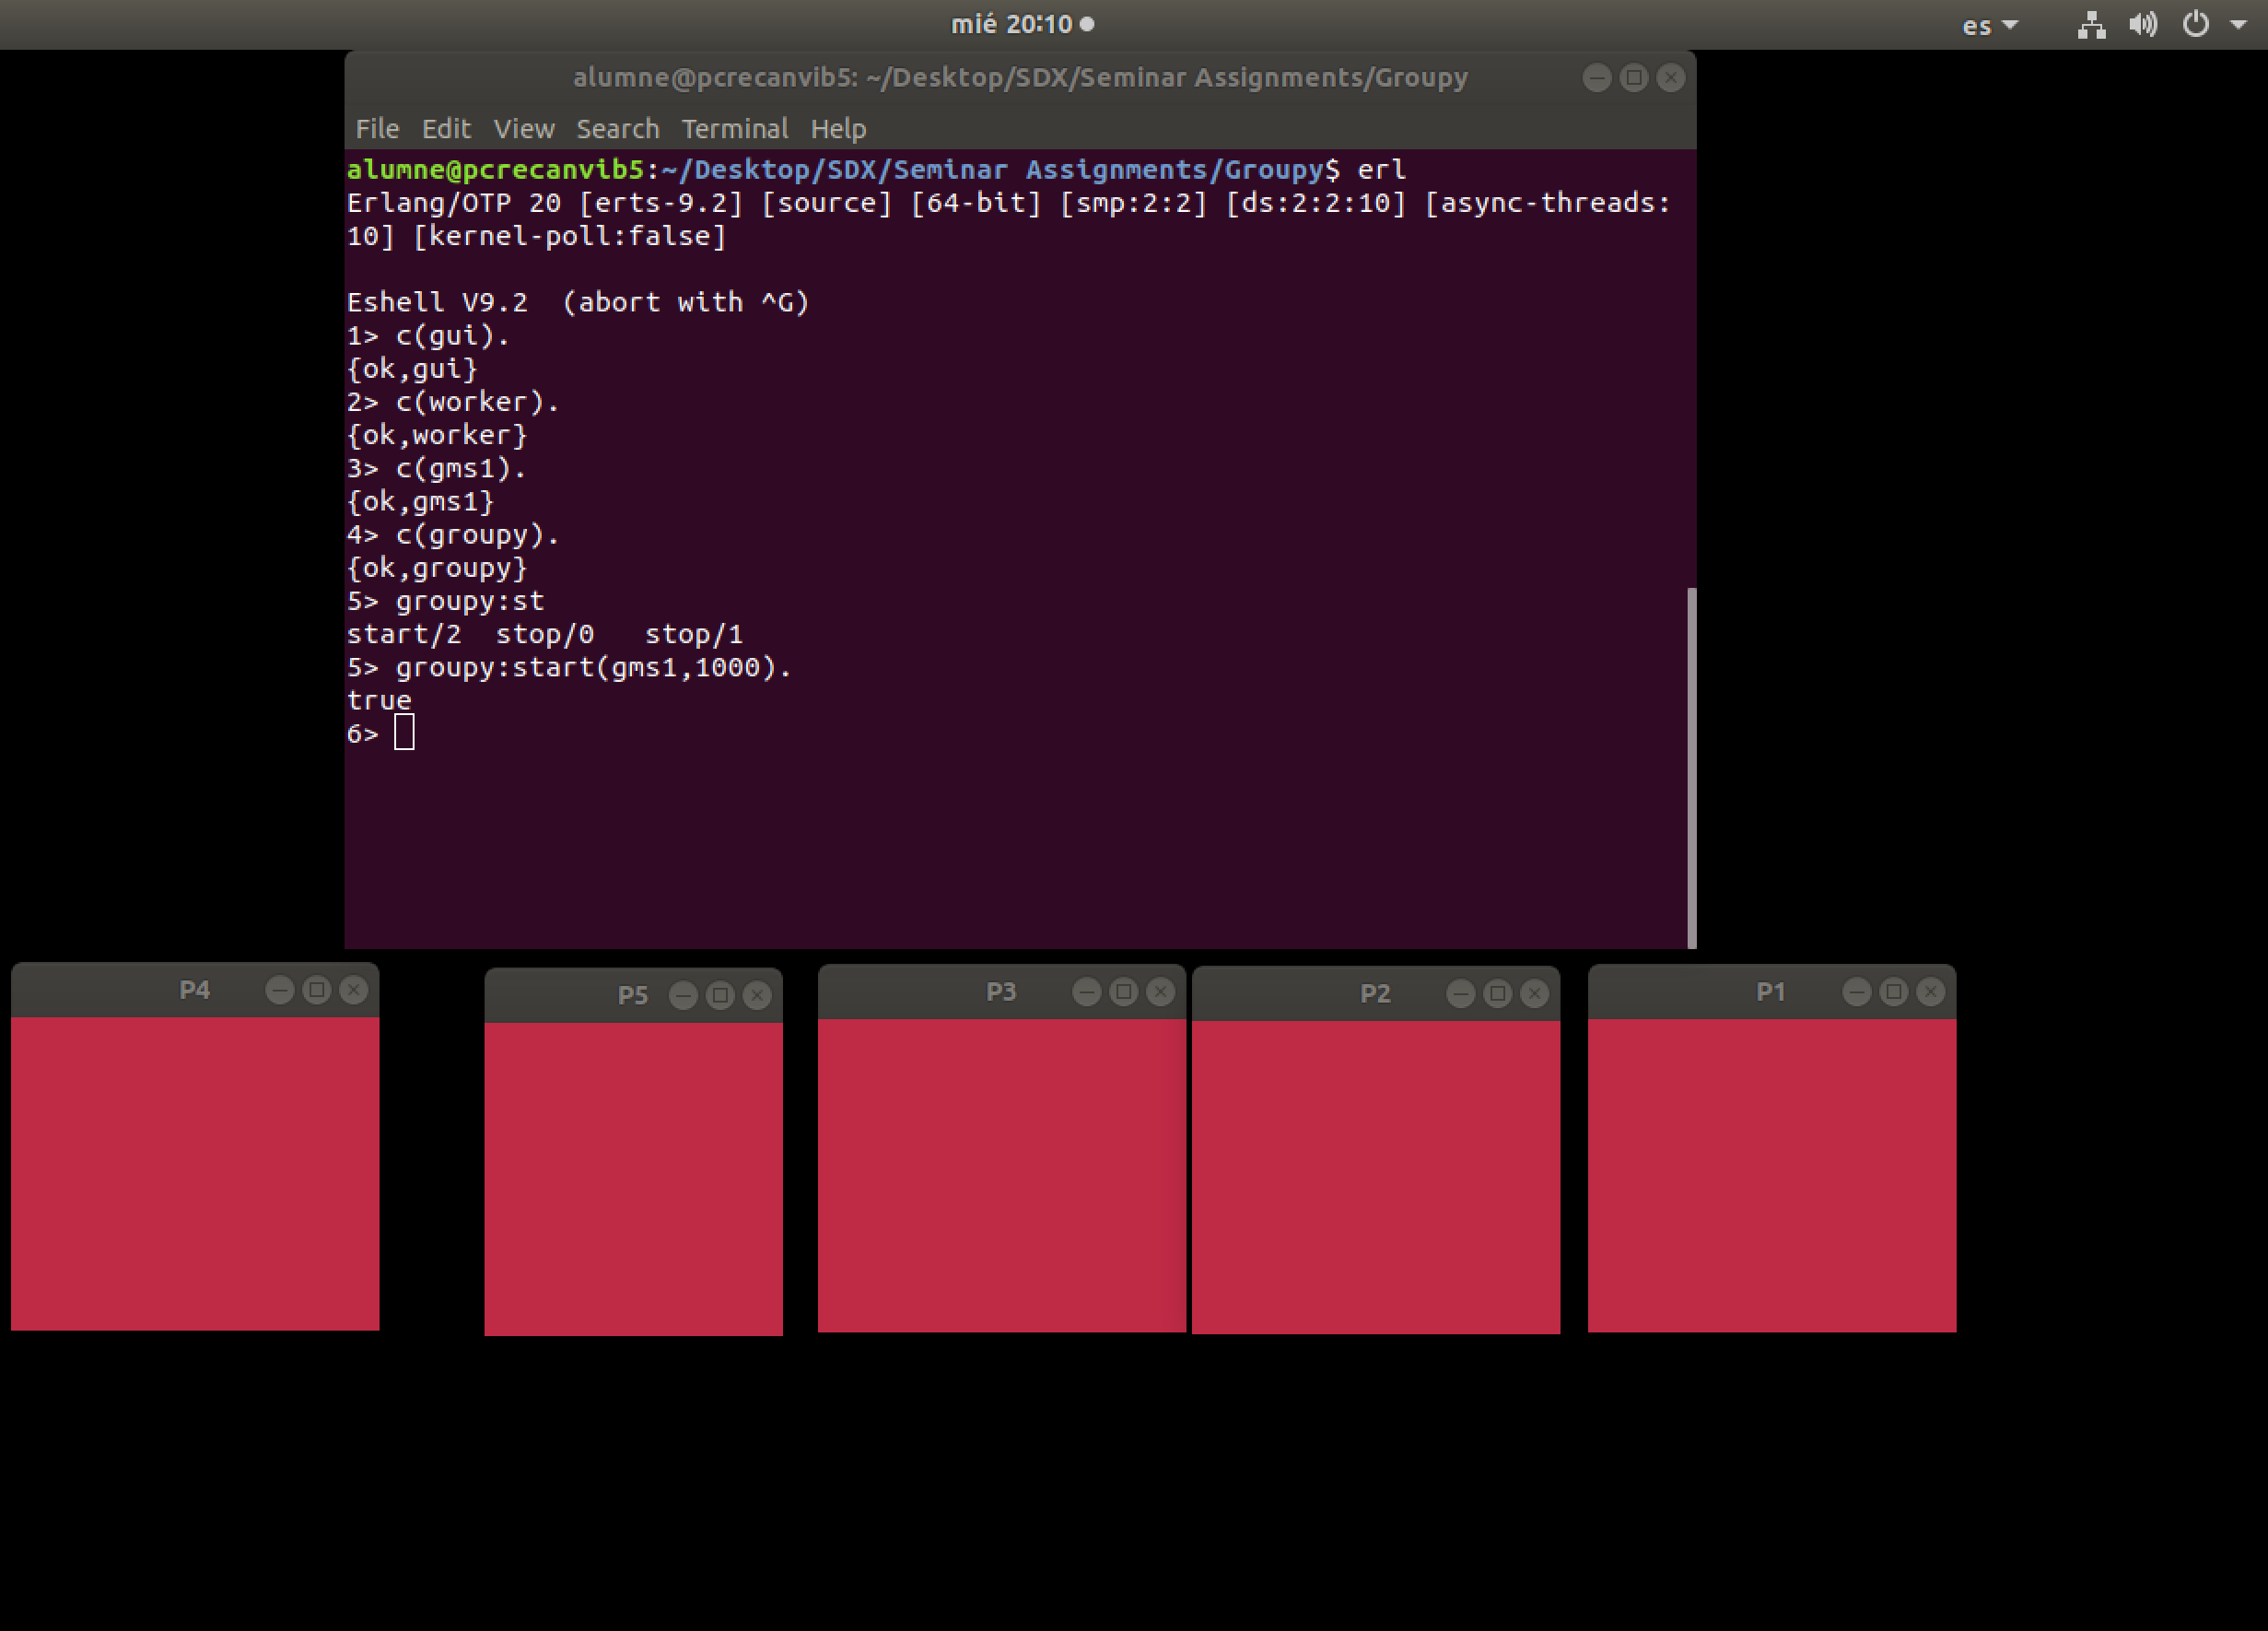
\includegraphics[width=\textwidth]{img1.png}\\\\
    Tal com observem a la figura, podem crear un grup i preservar el seu estat.\\
\newpage El segon objectiu d'aquest experiment és el de poder afegir nous nodes, que estiguin coordinats amb la resta. Per a tal fi, crearem un nou worker, que farà una request to join a un Slave, aquest reencaminara la petició al Lider del grup i so no hi ha cap fallada, el nou node passarà a formar part del grup com a Slave. Tal com podem veure a la figura següent:\\\\
    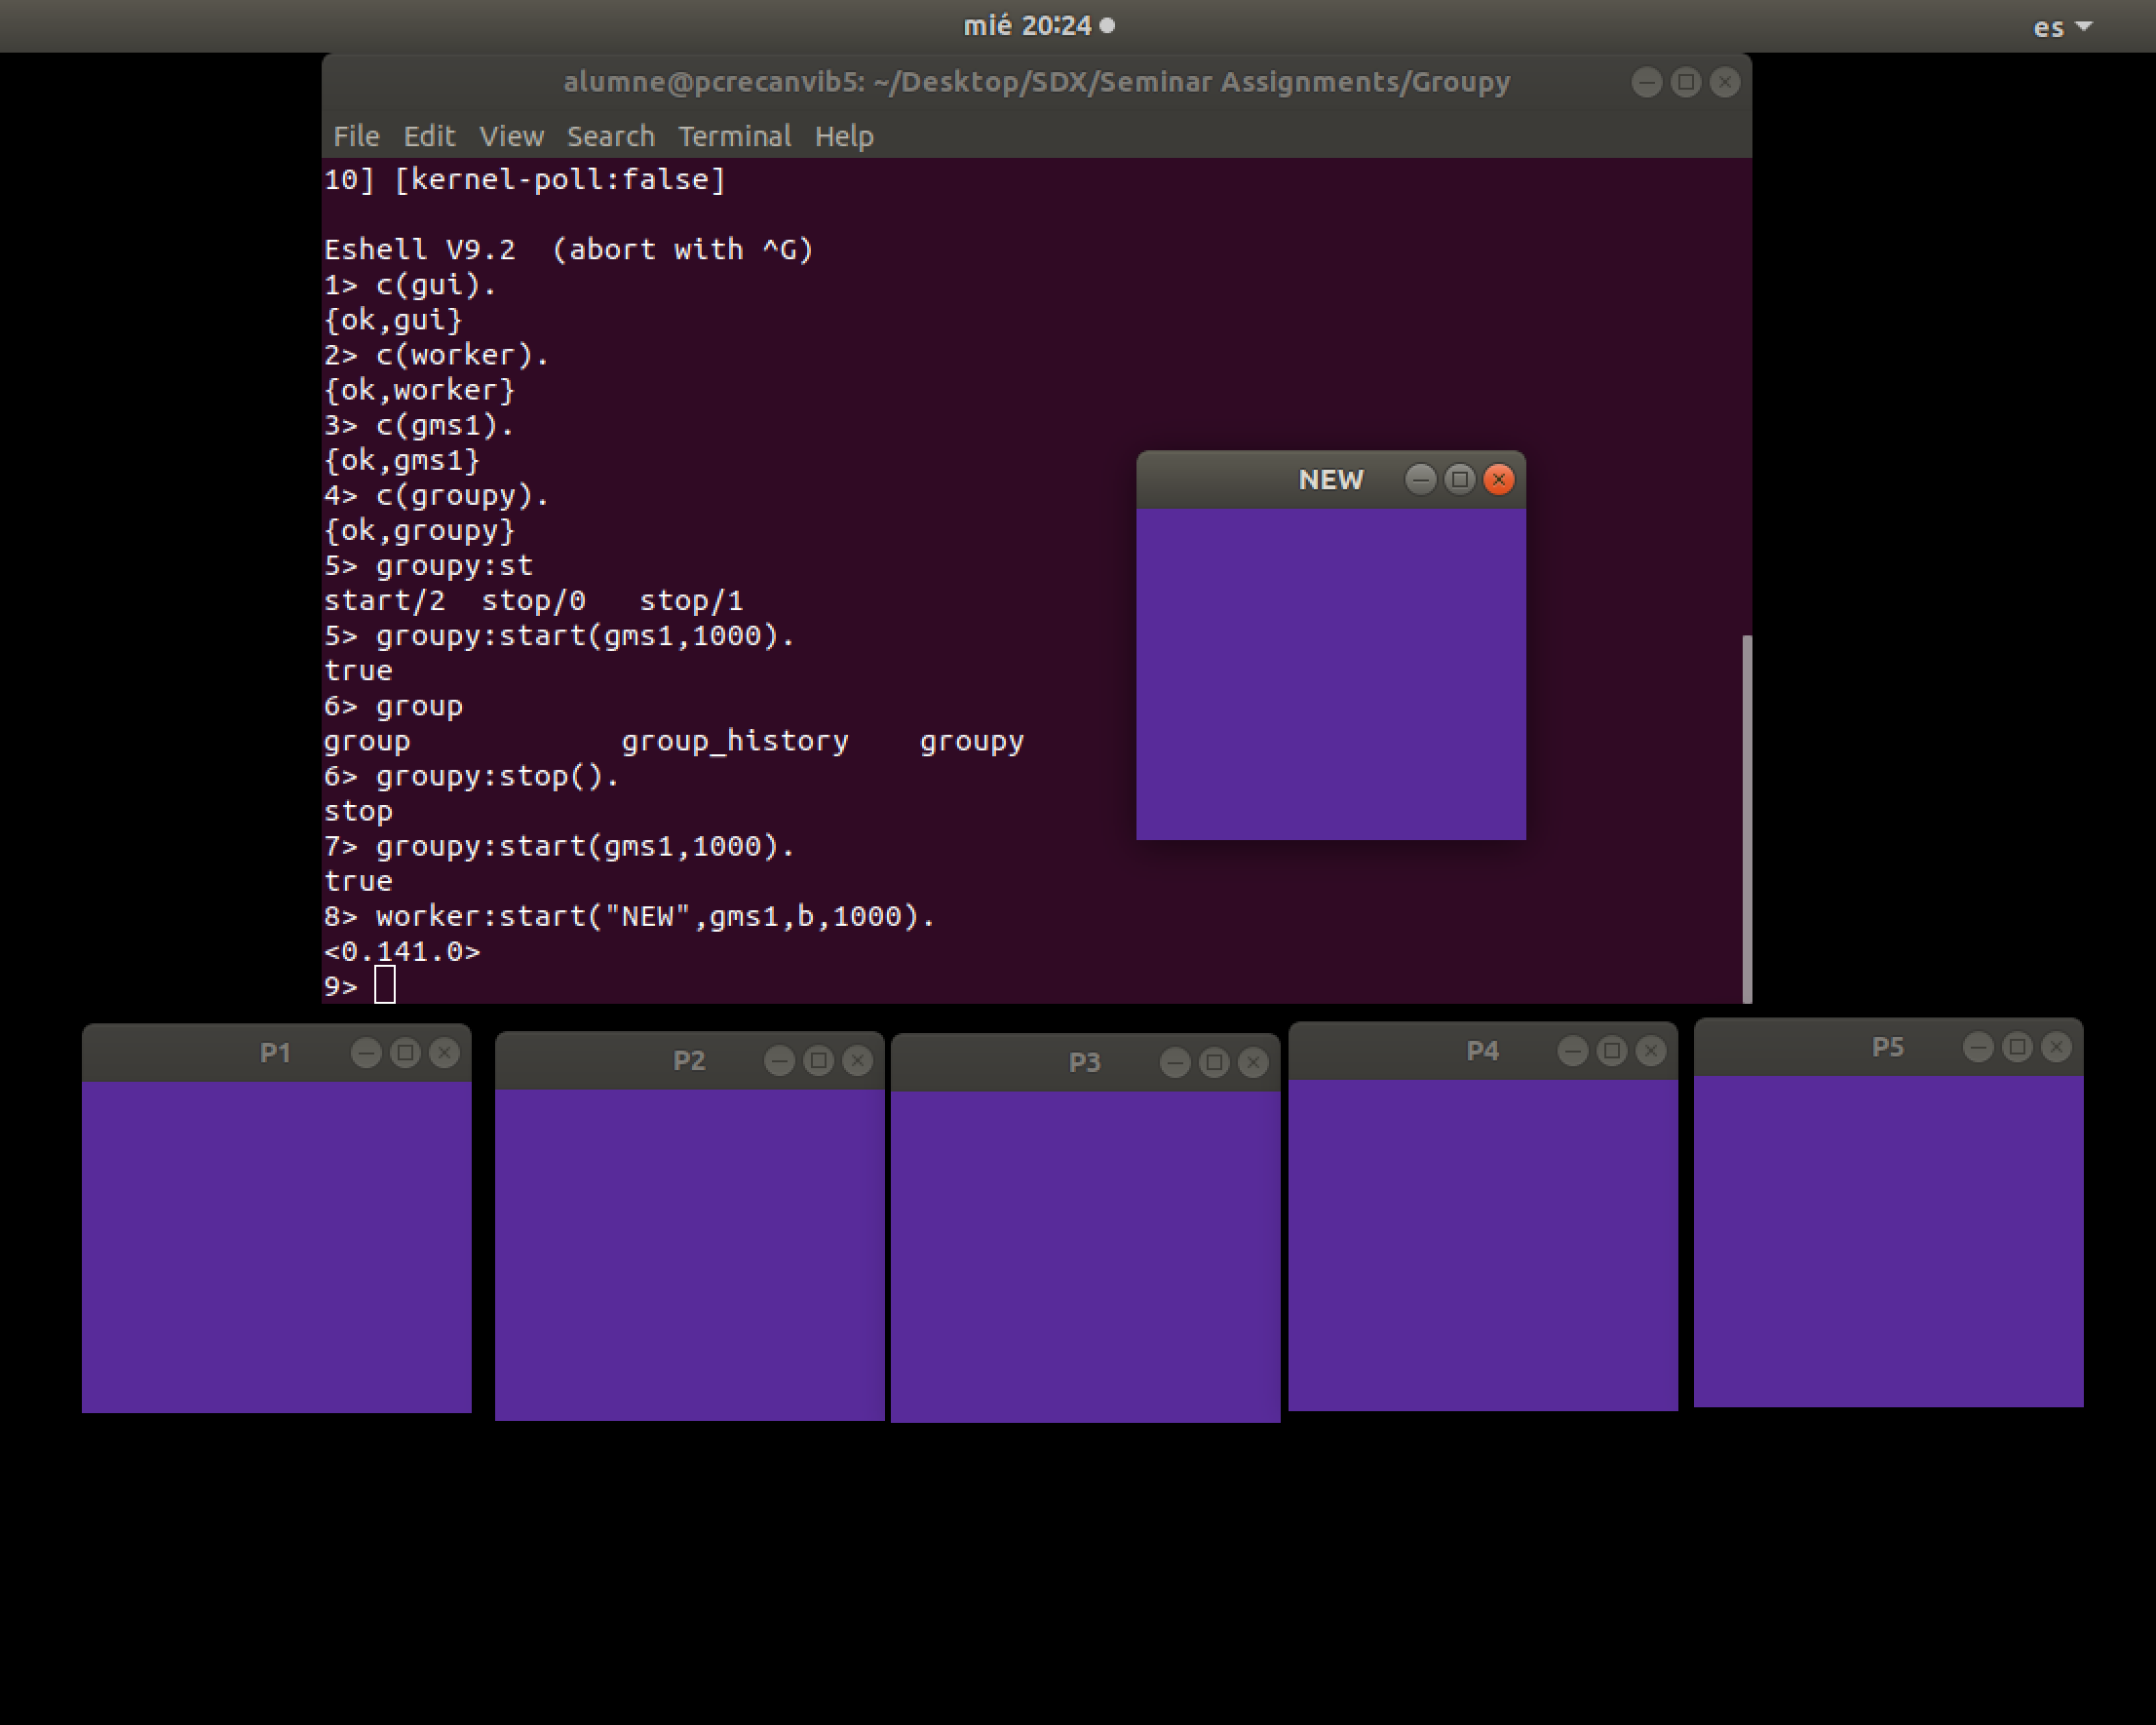
\includegraphics[width=\textwidth]{img2.png}

\newpage\item\textit{Adapt the groupy module to create each worker in
a different Erlang instance.}\\Per adaptar Groupy per tal de tenir cada worker en una instància erlang diferent, hem creat el fitxer groupyrem.erl, on tenim la implementació necessària per dur-ho a terme.\\
En la figura següent, podem veure com tot funciona correctament executant-se en diferents instàncies d'erlang:\\\\
    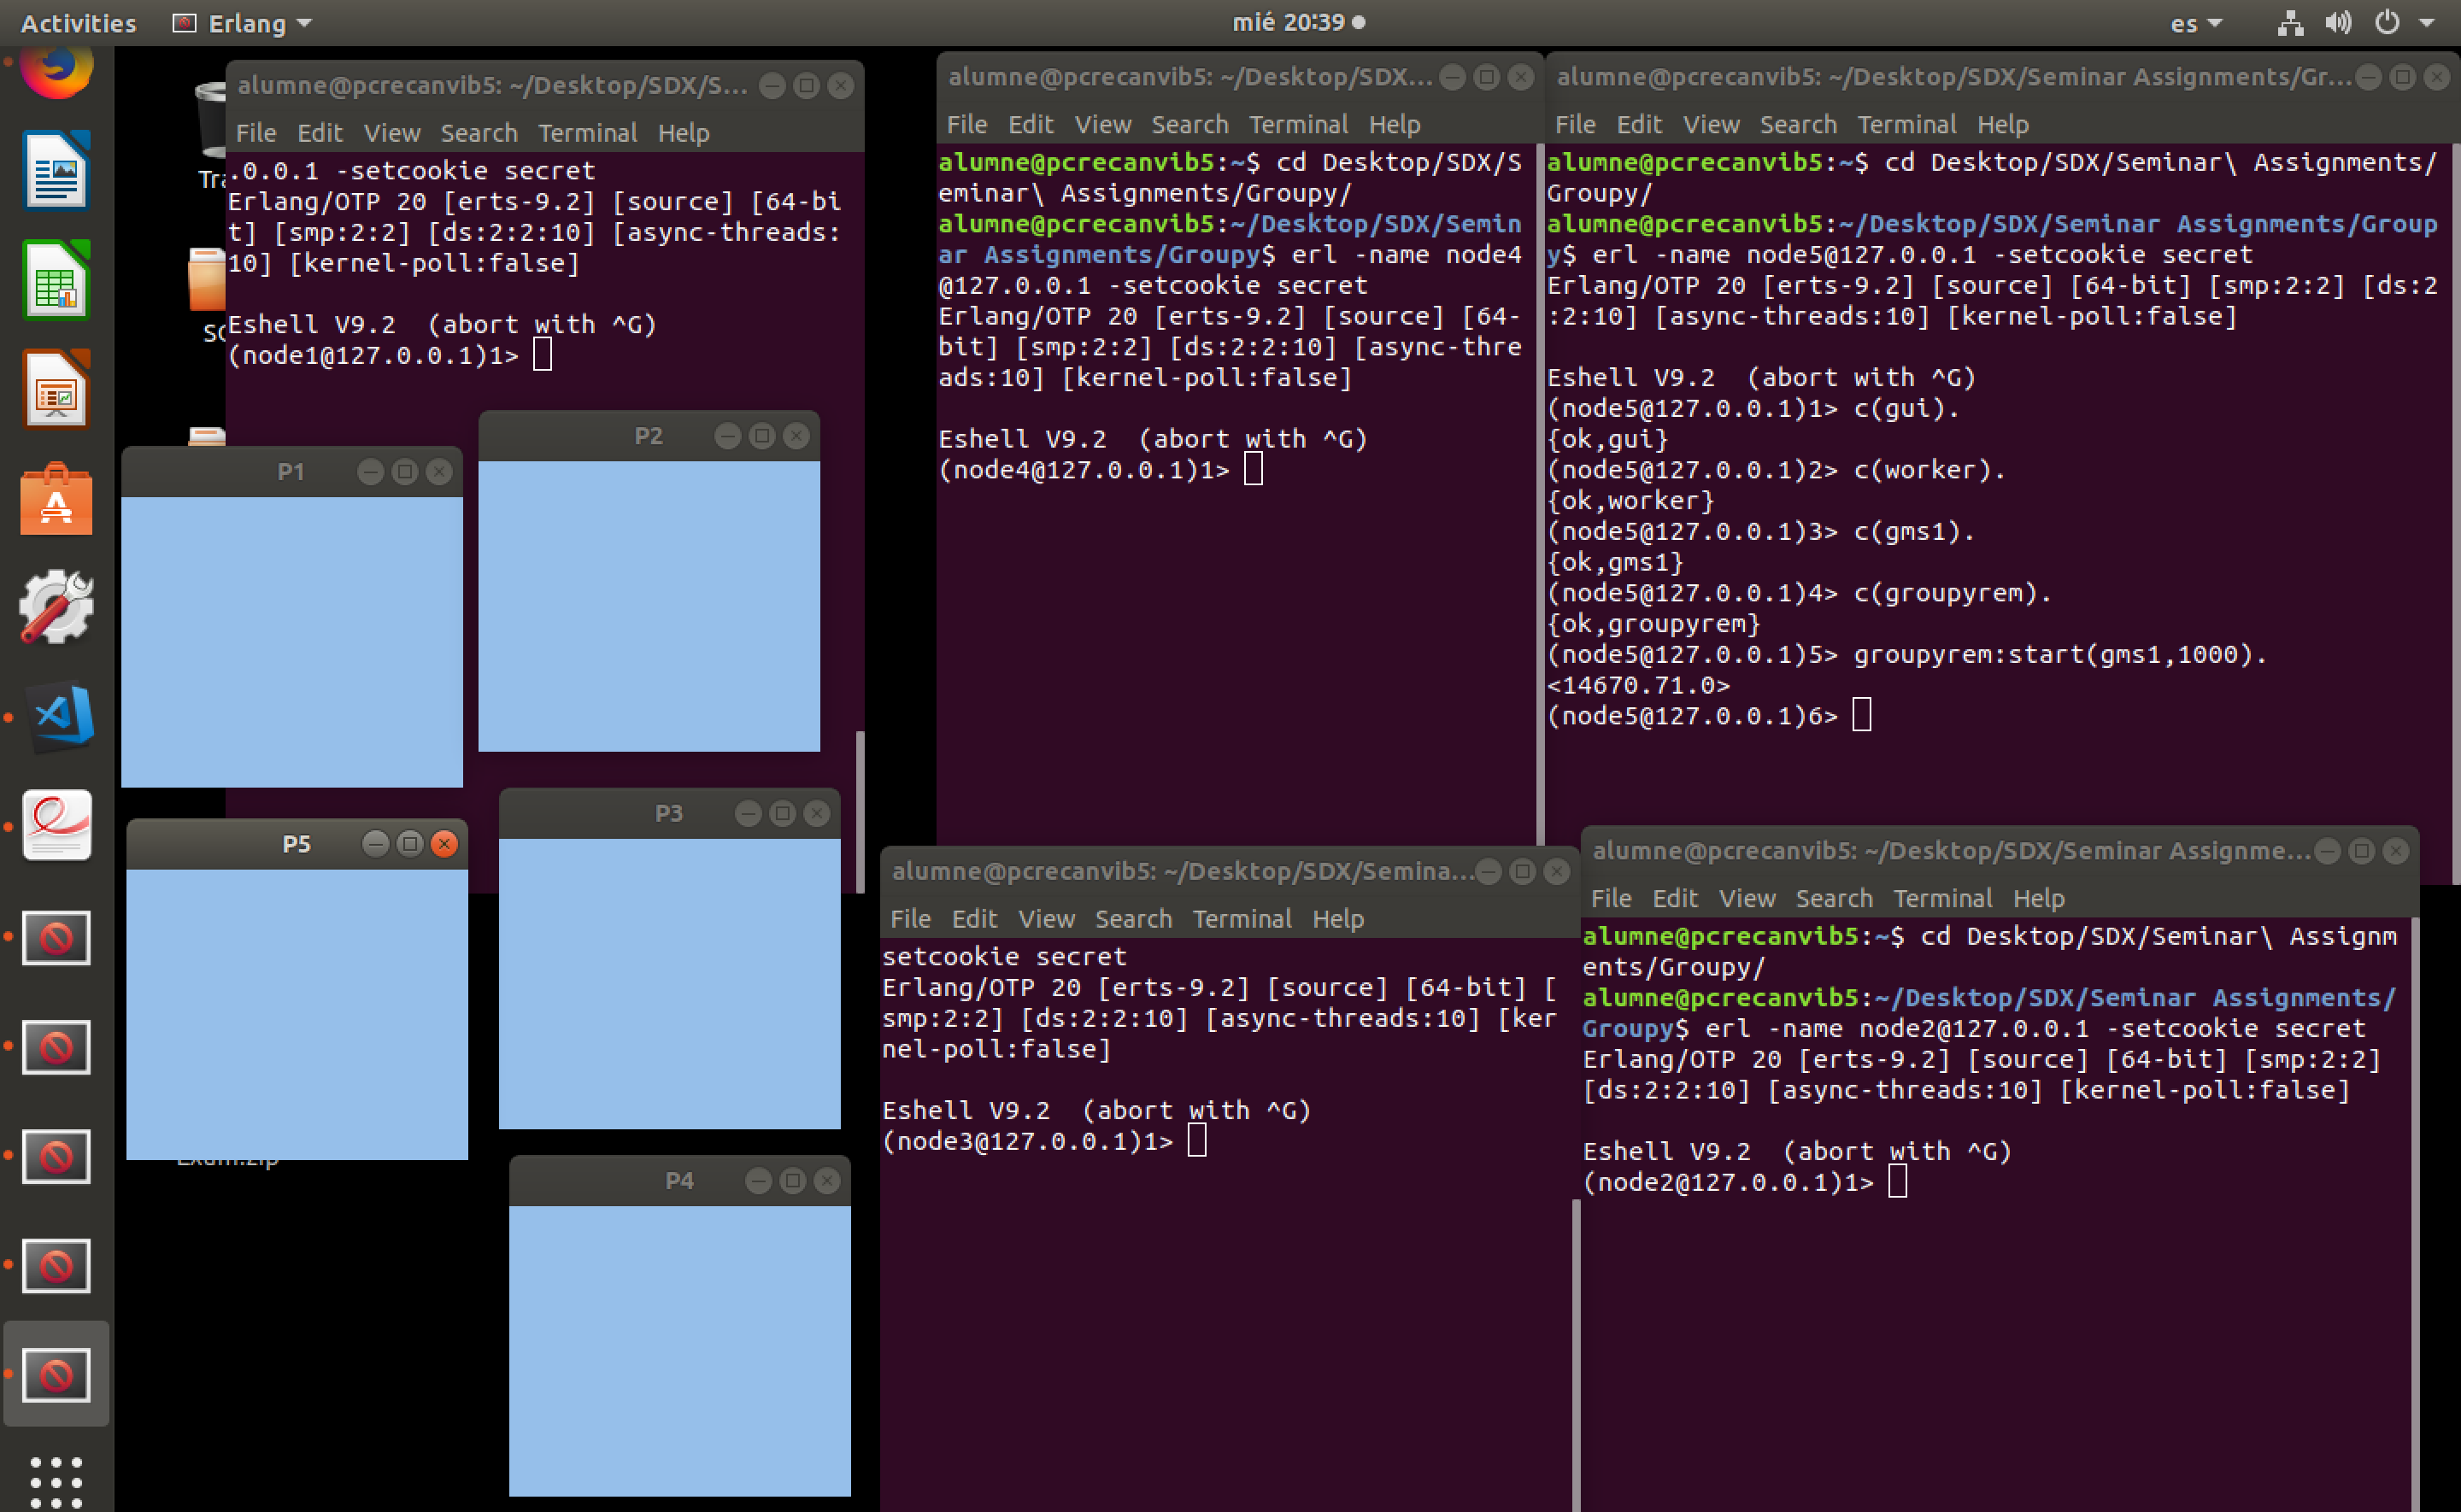
\includegraphics[width=\textwidth]{img3.png}
\end{enumerate}
\newpage\subsection{Handling Failures}
\subsection{Failure Detector}
\begin{enumerate}
    \item\textit{Do some experiments to see if the peers can keep their
state coordinated even if nodes crash.}\\Ara el nostre sistema distribuït hauria de ser capaç de suportar fallades.\\
Per provar-ho, experimentarem amb les diferents parts crítiques, com per exemple quan un Lider cau i s'ha de seleccionar un de nou.\\
Erlang ens permet monitorar processos, per la qual cosa quan els Slaves detecten que el Lider ha caigut, entraran en un estat d'elecció, del qual el primer Slave de la cua serà escollit com a nou Lider. En cas que els Slaves no hagin detectat que el Lider ha caigut, el nou Lider enviarà un multicast amb la nova vista. Tal com podem veure en la figura següent:\\\\
    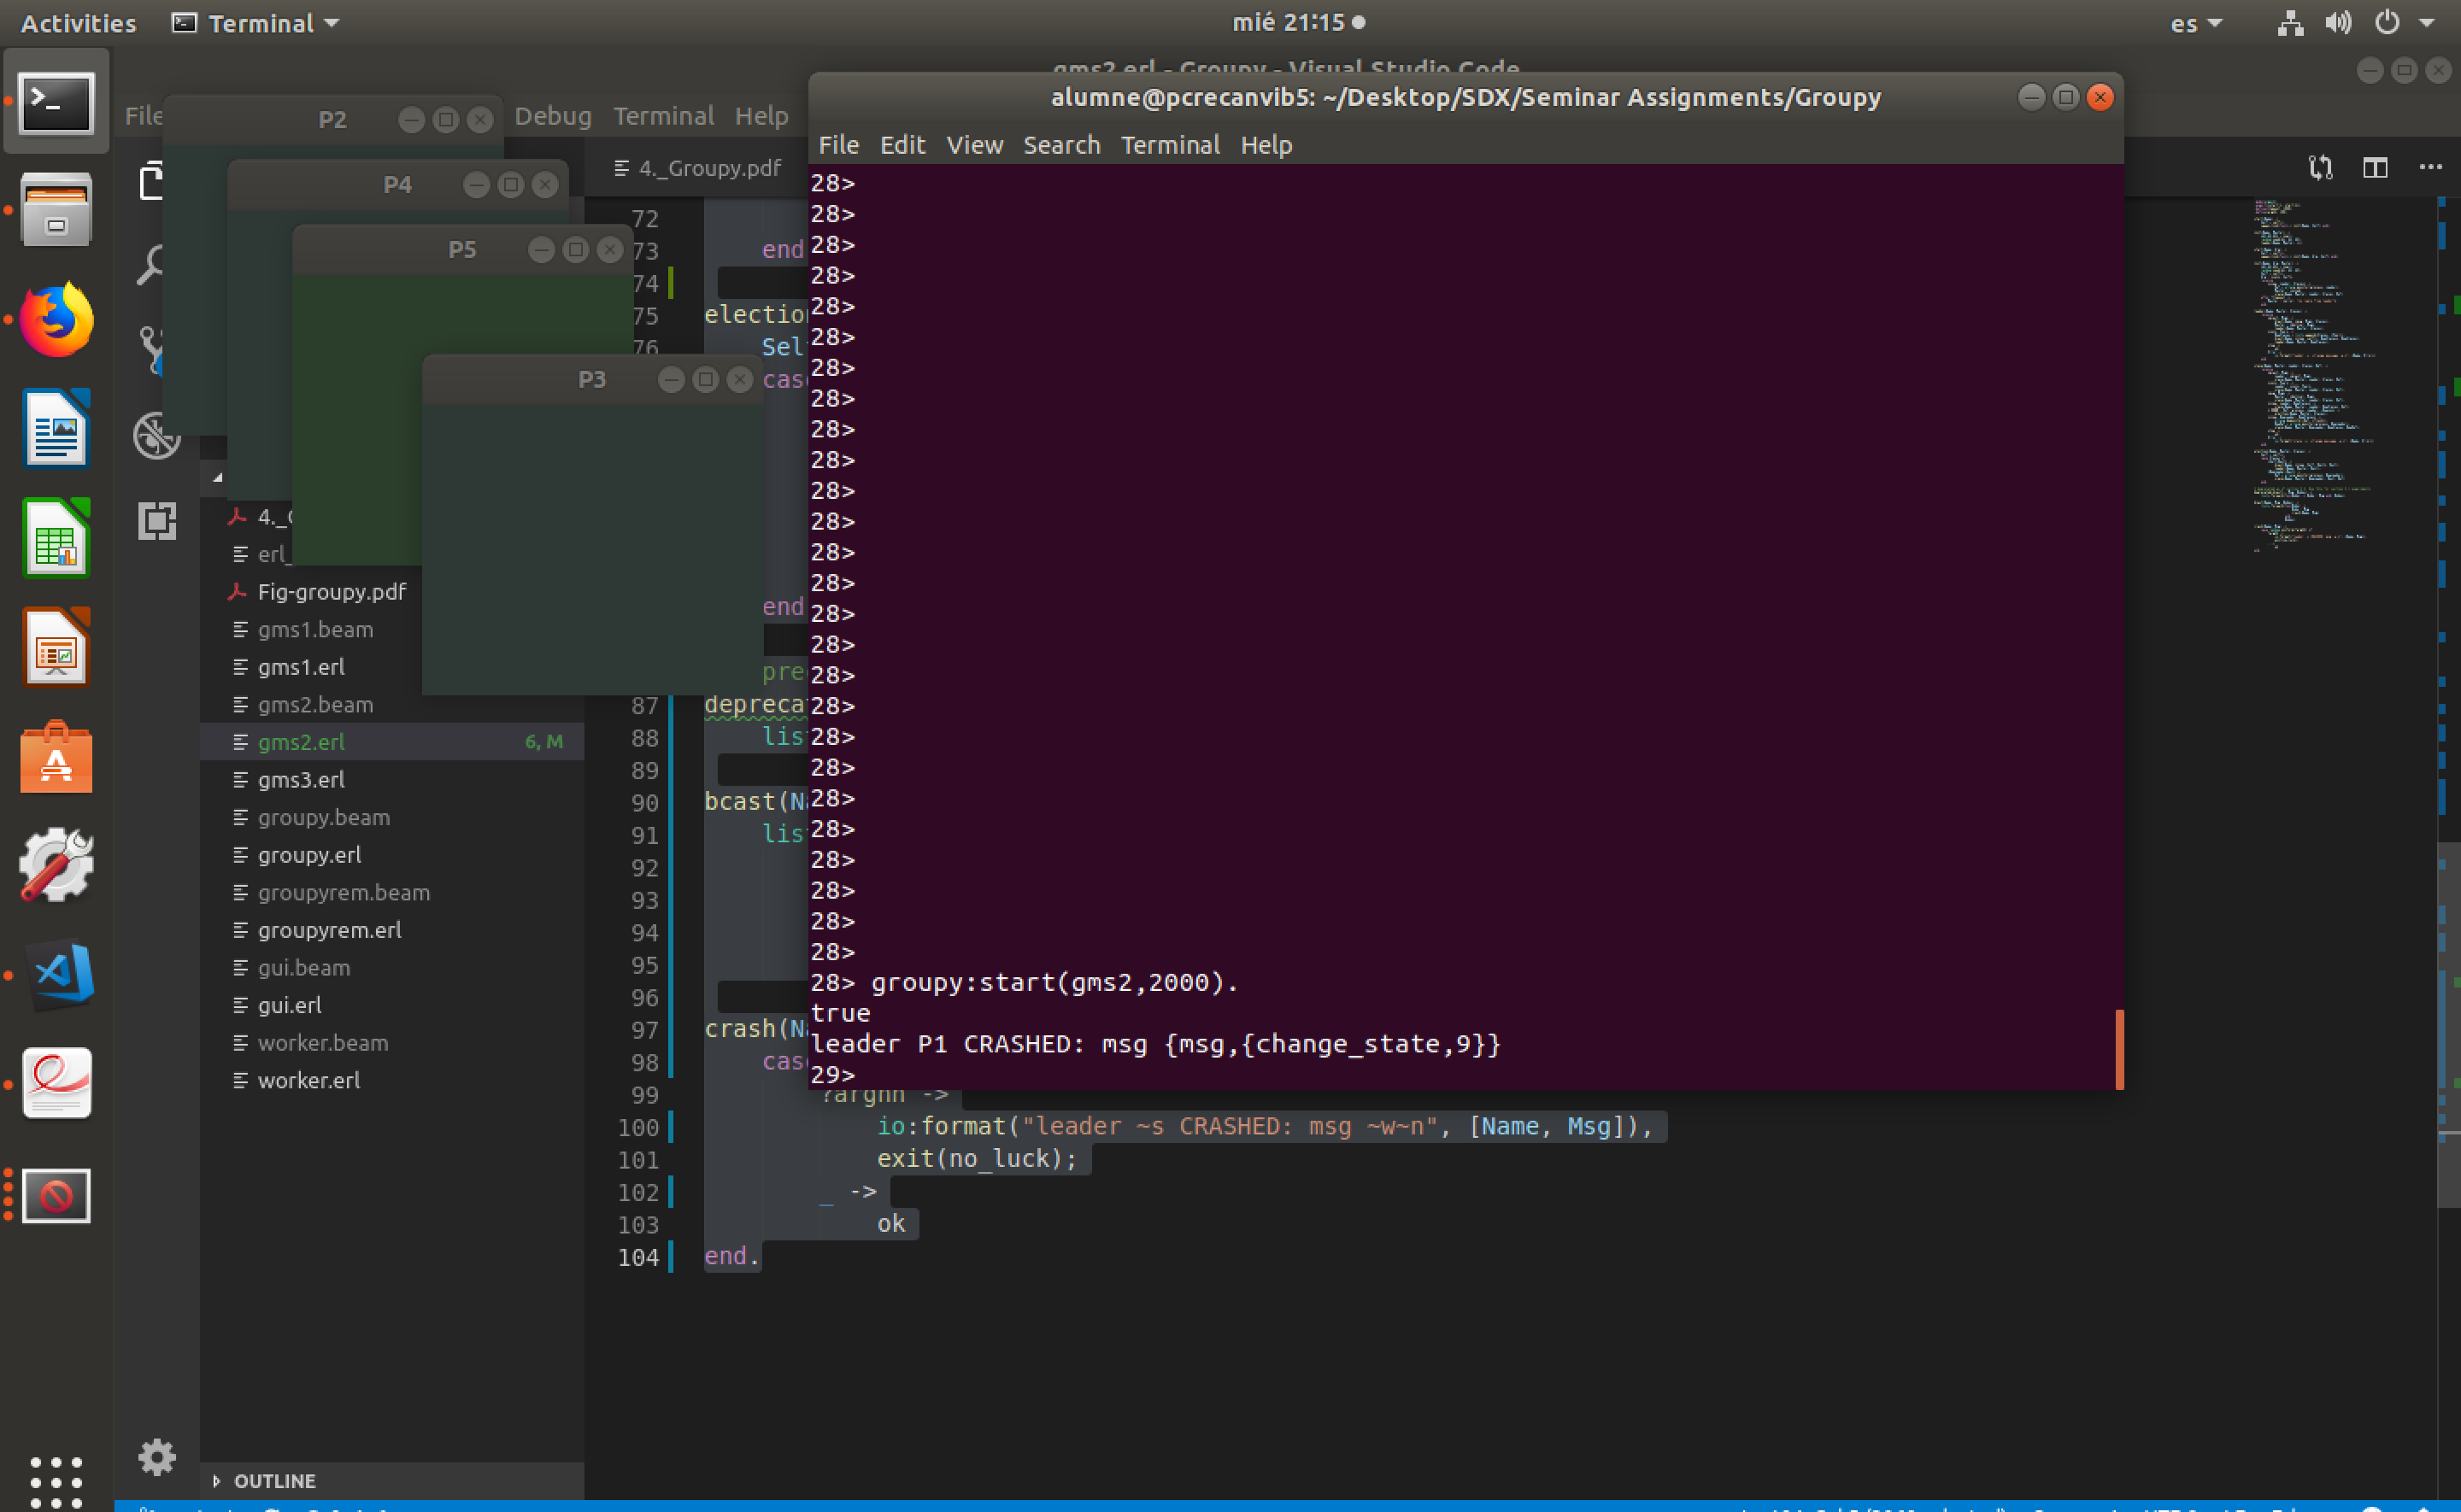
\includegraphics[width=\textwidth]{img4.png}\\\\
    Tal com es veu, el crash de Lider, no  afecta la coordinació del grup.\\
Així i tot, segueix existint una manera de què la coordinació del grup es pugui veure afectada, aquesta situació es donarà quan un Lider cau mentre està fent multicast, en elegir a un nou Lider, els Slaves poden quedar descordinats.\\
Per altra banda, si el que cau és un Slave, no hauríem de tenir cap problema de coordinació, ja que simplement aquest no rebrà els missatges que li siguin enviats i tampoc enviarà cap missatge al Lider.
\end{enumerate}
\newpage\subsection{Missing Messages}
\begin{enumerate}
    \item \textit{Repeat the experiments and see if you can have the state
of the workers become out of synch.}\\En aquesta execució, cada missatge té una probabilitat de pedres, de forma que tal com hem dit abans el grup, pot quedar descoordinat, tal com podem observar ala figura següent:\\\\
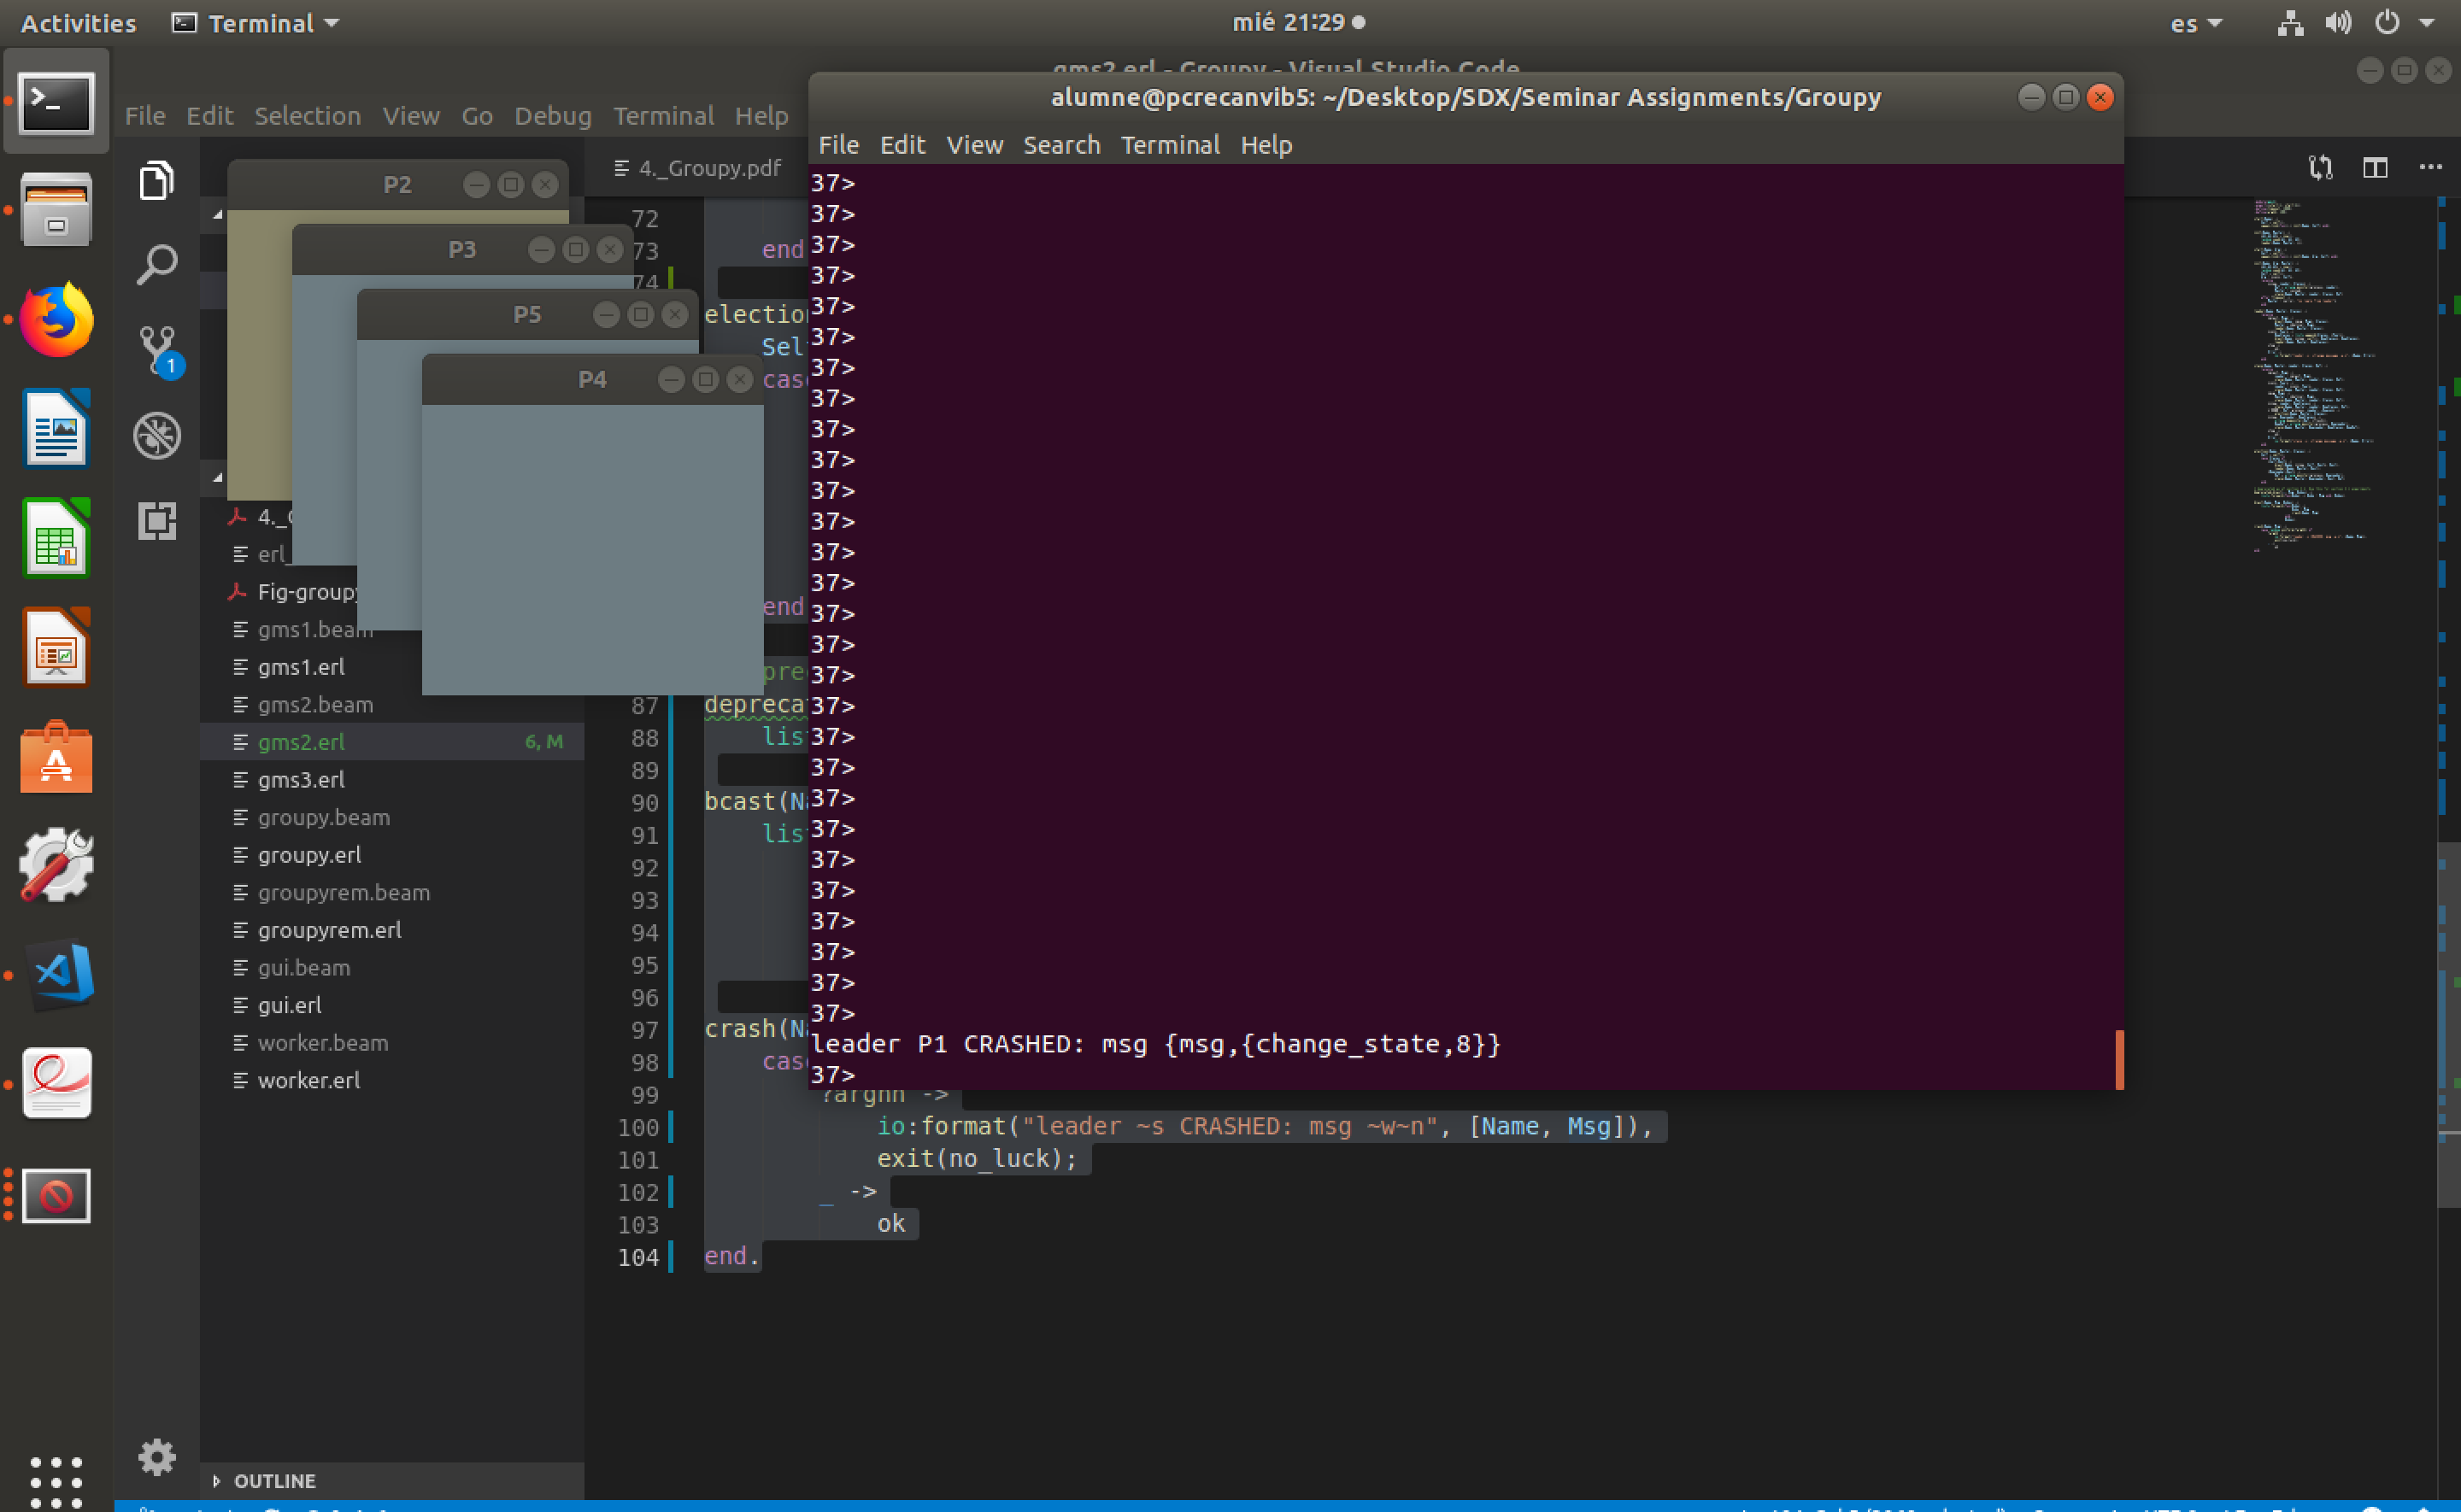
\includegraphics[width=\textwidth]{img5.png}\\\\
Per tant podem concloure que el nostre sistema encara no és completament a prova de fallades.
\end{enumerate}
\newpage\subsection{Reliable Multicast}
\begin{enumerate}
    \item \textit{ Repeat the experiments to see if now the peers can keep their state coordinated even if nodes crash.}\\
    Ara el nostre sistema sí que serà completament tolerant a fallades, ja que no existeix la possibilitat que a l'elegir un nou Lider es descoordini el grup. Tal com podem observar ala figura següent:\\\\
        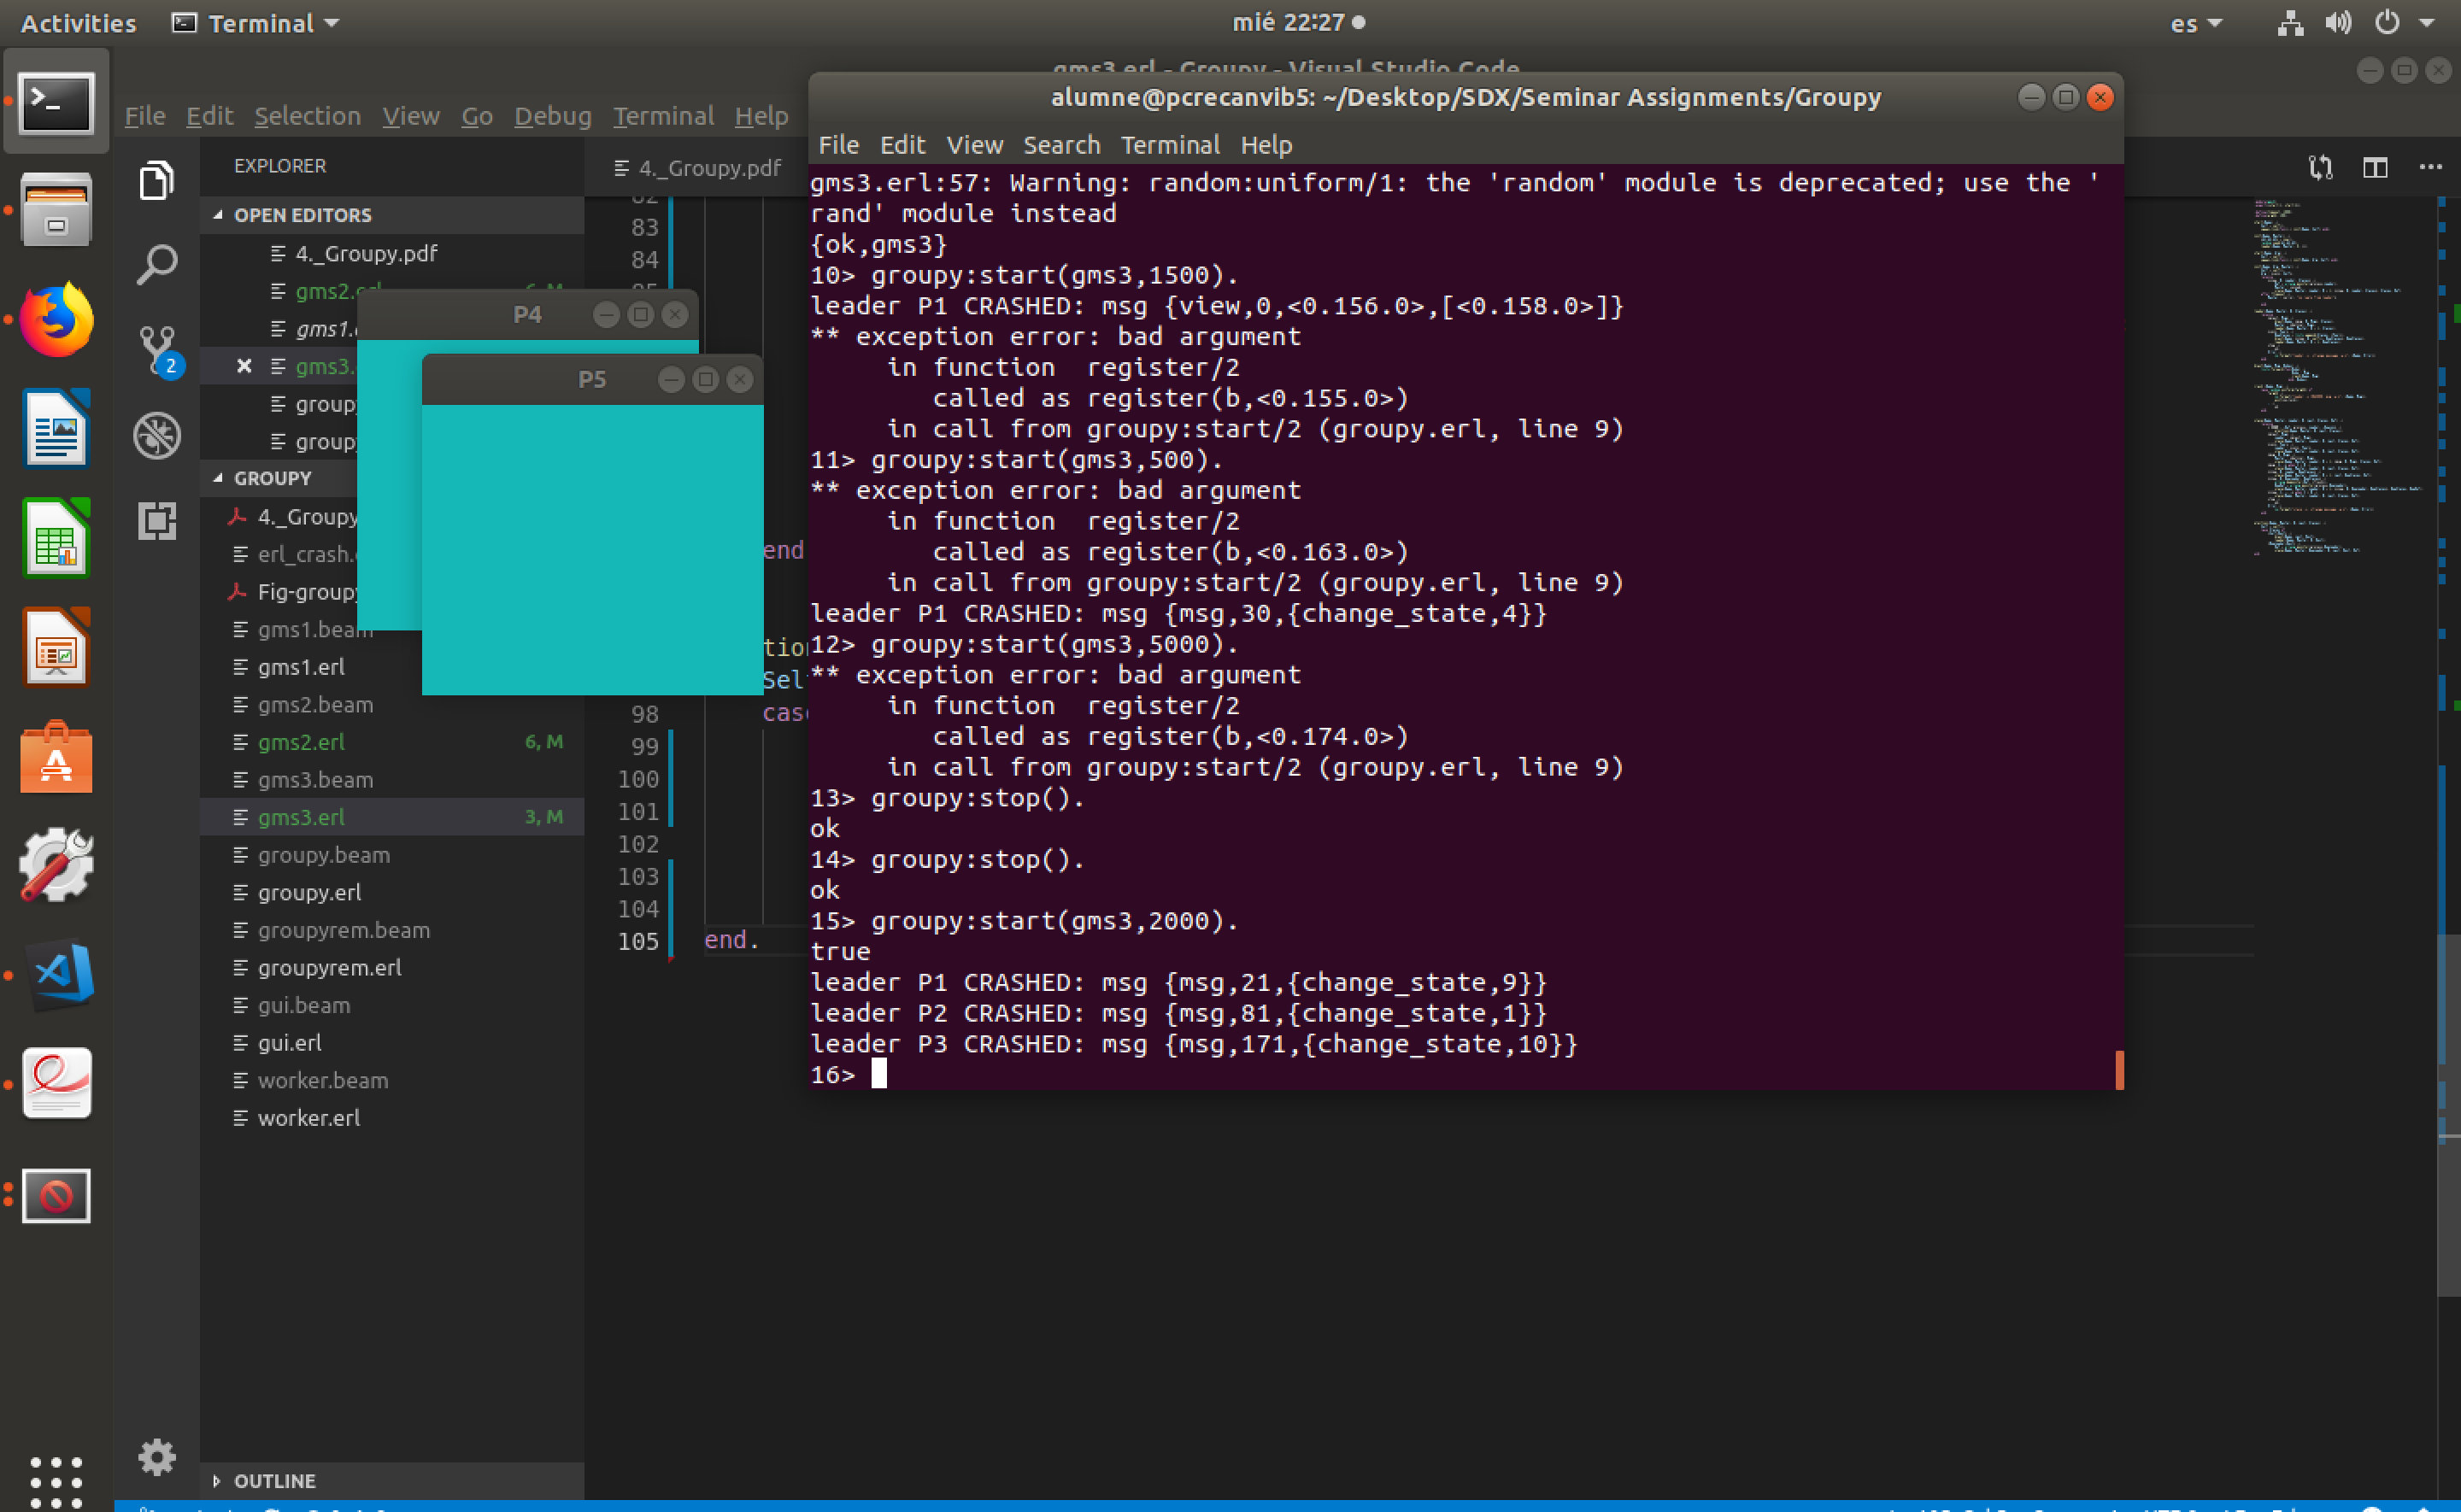
\includegraphics[width=\textwidth]{img6.png}\\\\

 \item \textit{ Try to keep a group rolling by adding more nodes as existing nodes die.}\\
 En aquest experiment fem que quan el Lider cau, afegeixi un nou node al grup, de forma que mai ens quedarem amb un grup d'un sol worker.
\end{enumerate}

\newpage\section{Open Questions}
\begin{enumerate}
    \item\textit{Why do the workers desynchronize?}\\
    Això el causa la fallada del leader abans d'acabar d'enviar els missatges multicast, ja que només una porció dels slaves rebran aquest últim missatge, donant lloc a que el worker respectiu no tindrà disponible el canvi de vista/color correcte. I quedarà dessincronitzat.
    \item\textit{How would we have to change the implementation to handle the possibly lost messages?}\\
    Per resoldre el problema dels missatges perduts, haurem d'utilitzar algun mecanisme de reliable multicast. Com basic reliable multicast, enviant ACK al líder per tal de mantenir un control dels missatges enviats i així que el lider no canvies d'estat fins que rebi tots els ACK corresponents, d'aquesta manera minimitzaríem la dessincronització a un únic color.
En el cas de canvi de líder, no podem estar segurs que el següent de la llista, per convertir-se en líder , hagués rebut tots els missatges i tornar a reenviar als slaves en cas necessari. Per aquest motiu una possible solució seria implementar un procés d'elecció que prioritzes nodes que tinguin disponibles missatges amb el màxim número de seqüència, per tal que el reliable multicast funcioni.\\
    \newpage\item \textit{How would this impact performance?}\\
La nostra solució de basic reliable multicast haurà de doblar el nombre de missatges, ja que cada slave haurà d'enviar un ACK, a més el líder haurà d'esperar un RTT sencer en cas de no rebre tots el ACK i fer el canvi d'estat.

    \item \textit{What would happen if we wrongly suspect the leader to have crashed?}\\
    Amb la implementació del sistema actual, ja tindrem present un nou Leader. Els Slaves envien peticions multicast a aquest nou Leader però l'antic continuarà gestionant les peticions de canvi d'estat del seu worker, amb qui continuarà fent multicast.\\
    La resta de nodes del sistema (Leader + Slaves) processaràn aquests canvis d'estat ja que no es pot saber que el missate de canvi d'estat sigui emès pel Leader. Els Workers estaràn sincronitzats ja que rebran els mateixos missatges. L'únic que no funcionarà d'acord a la nova implementació és el Worker associat a l'anterior Leader. Aquest no hi serà a la llista de la resta i només respondrà a les seves propies peticions.\end{enumerate}

\section{Personal opinion}
    Aquest laboratori ha ajudat a clarificar un dels conceptes més comuns dels sistemes distribuïts en xarxa: La communicació multicast. Mitjançant la pràctica de l'implementació de nodes com poden ser els Workers, Leaders i Slaves, es té una visió més exemplificadora del problema que s'ha tractat.
\end{document}
